
%----------------------------------------------------------------------------------------
%   Хавсралтууд эндээс эхэлнэ
%----------------------------------------------------------------------------------------
\appendix
\addcontentsline{toc}{part}{ХАВСРАЛТ}

% Хавсралтын нэр. Хавсралт гэдэг үг агуулахгүй
\chapter{Үечилсэн төлөвлөгөө}
\begin{figure}[ht]
	\centering
	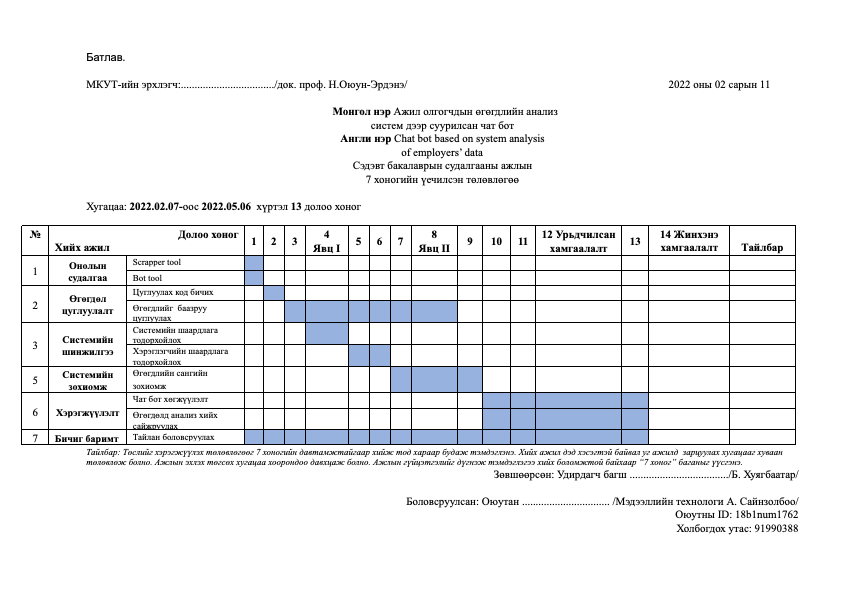
\includegraphics[width=16.5cm, angle=90]{images/plan.png}
	\caption{Бакалаврын судалгааны ажлын үечилсэн төлөвлөгөө}
	\label{fig:plan01}
\end{figure}
% Хавсралтын нэр. Хавсралт гэдэг үг агуулахгүй
\chapter{Кодын хэрэгжүүлэлт}

\section{Өгөгдөл цугуулалт}
Өгөгдөл цуглуулах програм нь дараах бүтэцтэй байх бөгөөд assets доторх кодууд нь үндсэн кодыг ажлуулахад туслах функцууд байна.
\begin{figure}[ht]
	\centering
	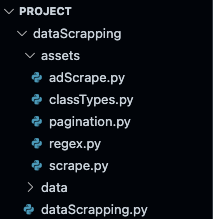
\includegraphics[width=5cm]{images/folderStructure.png}
	\caption{Фолдерийн бүтэц}\label{fig:folderStructure}
\end{figure}
\subsection{Үндсэн өгөгдлийг цуглуулах}
\lstinputlisting[language=Python, caption=Бүх өгөгдлийг цуглуулах - dataScraping.py]{code/dataScrapping.py}
\subsection{Нэг зарын шаардлагатай бүх мэдээллийг цуглуулах}
\lstinputlisting[language=Python, caption=Нэг зарын өгөгдлийг цуглуулах - adScrape.py]{code/adScrape.py}
\subsection{Цуглуулах өгөгдлийн төрөл}
\lstinputlisting[language=Python, caption=Өгөгдлийн төрөл - classTypes.py]{code/classTypes.py}
\subsection{BeautifulSoup scraper}
\lstinputlisting[language=Python, caption=Scrape хийх функц - scrape.py]{code/scrape.py}
\section{Өгөгдөл нэгтгэх, цэвэрлэх}
\lstinputlisting[language=Python, caption=Өгөгдөл цэвэрлэх - dataClean.py]{code/cleanData.py}

\section{Өгөгдлийн сангийн холболт}
\subsection{Өгөгдлийн санг удирдах}
ORM ашиглан виртуал машин дээрх өгөгдлийн сантай харьцна.
\lstinputlisting[language=Python, caption=Elastic IP-руу холбогдох - connection.py]{code/connection.py}
\subsection{Өгөгдлийн сантай харьцах}
\lstinputlisting[language=Python, caption=Өгөгдлийн сангийн зохиомж болон upsert функц - upsert.py]{code/insert.py}
\section{Чатбот хөгжүүлэлт}
\subsection{Үндсэн чатбот удирдлага}
\lstinputlisting[language=Python, caption=чатбот класс - bot.js]{code/chatbotCode/bot.js}
\subsection{API helper}
\lstinputlisting[language=Python, caption=Өгөгдлийн сангаас өгөгдөл авах - apiHelper.js]{code/chatbotCode/apiHelper.js}
\subsection{Question Understand}
\lstinputlisting[language=Python, caption=Хэрэглэгчийн асуултыг ойлгох\, query үүсгэх - questionUdnerstand.js]{code/chatbotCode/questionUnderstand.js}
\subsection{Card Builder}
\lstinputlisting[language=Python, caption=Хэрэглэгчид харагдах байдлыг угсрах - cardBuilder.js]{code/chatbotCode/cardBuilder.js}